\subsection{Modelo de comportamiento}

\subsubsection{Diagrama de actividad}

En este ultimo modelo mostraremos las actividades realizadas con su respectivo orden. Este orden lo indicaremos con flechas. También mostraremos los responsables de cada actividad. Las actividades también pueden suceder de forma concurrente. Para esto usaremos una barra (que llamaremos fork) y colocaremos las actividades concurrentes debajo de esta. Luego de esto hace falta que las actividades esperen a las que iniciaron el fork con ésta. Usaremos también una barra para esto, colocando las actividades por encima (que llamaremos join). Además se colocará condiciones if que indican a dónde se dirigirá un flujo que depende de esa condición.

Los flujos que se observan son:
\begin{itemize}
\item El flujo de un pedido de un cliente y de un local desde que es realizado hasta que es entregado o no a su domicilio.
\item El flujo de reponer el stock de un depósito desde que se arma el pedido para el proveedor hasta que este los envía y se actualiza el stock en consecuencia.
\end{itemize}

En estos tres flujos se puede observar el orden en el que son realizados muchos de los casos de uso que se mostraron en el primero modelo.

A continuación presentamos los tres diagramas de actividad realizados:

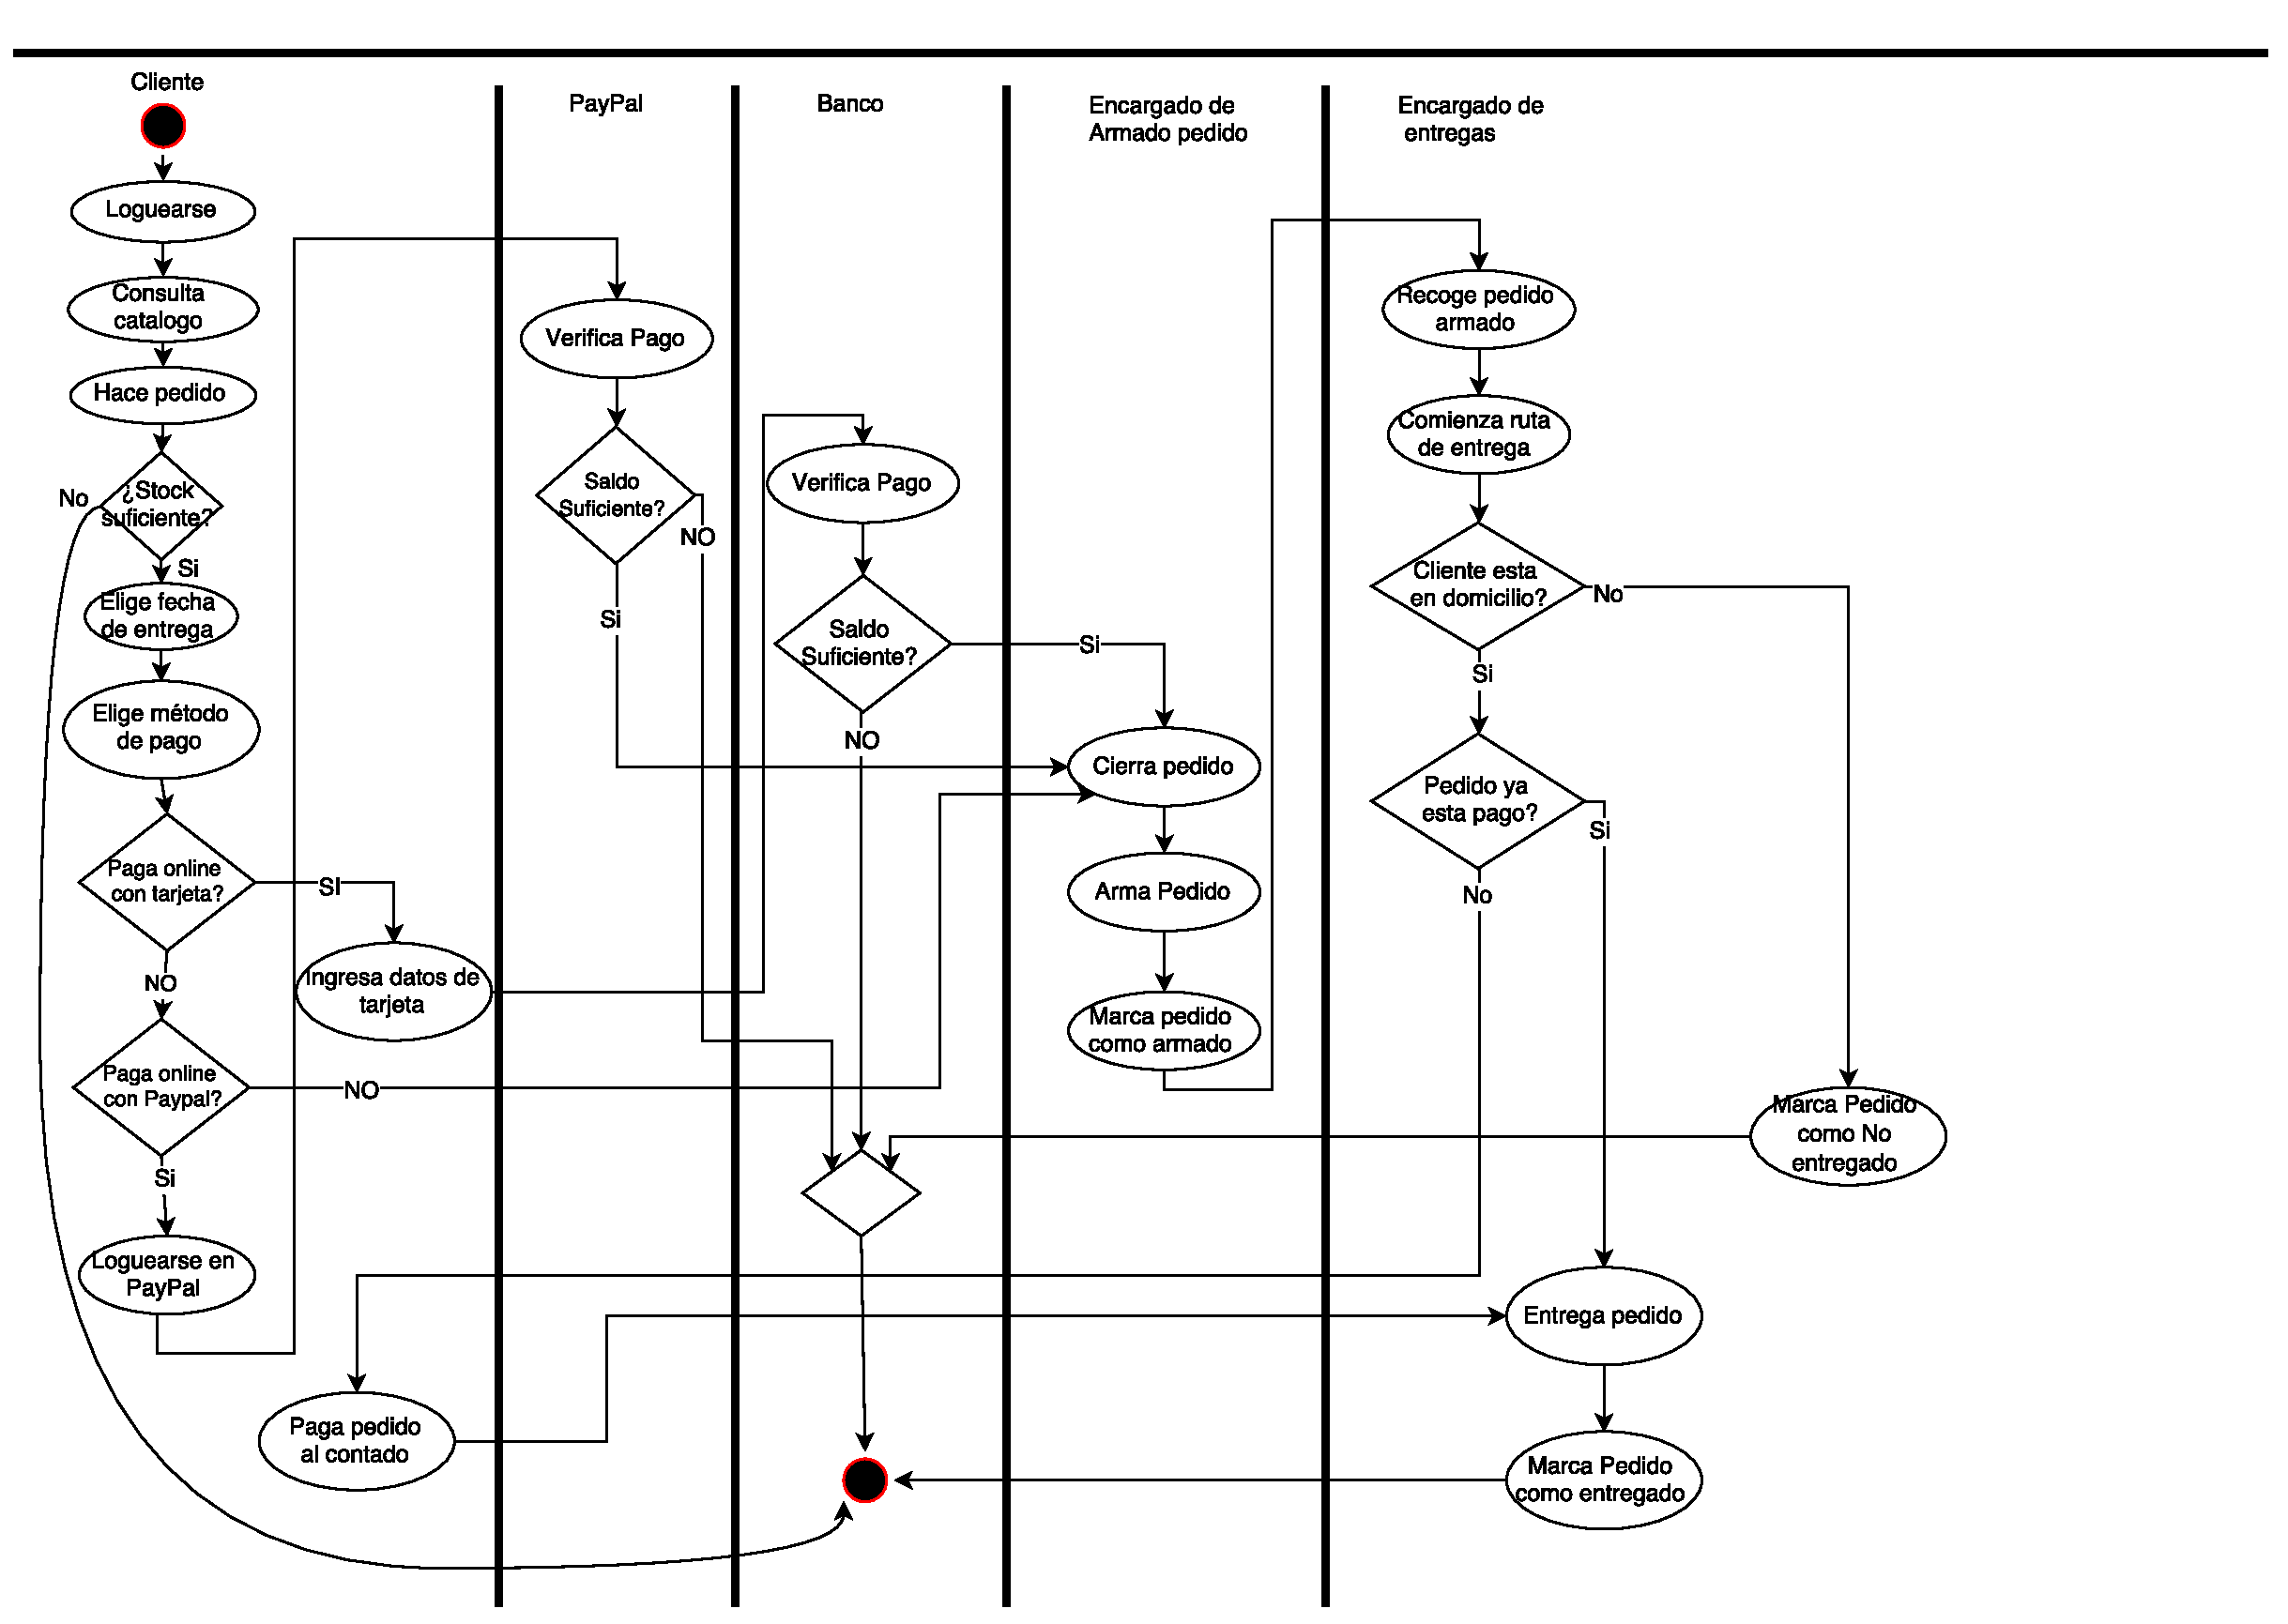
\includegraphics[scale=0.5, angle=90]{secciones/diagramaActividad1}
\newpage
\newpage
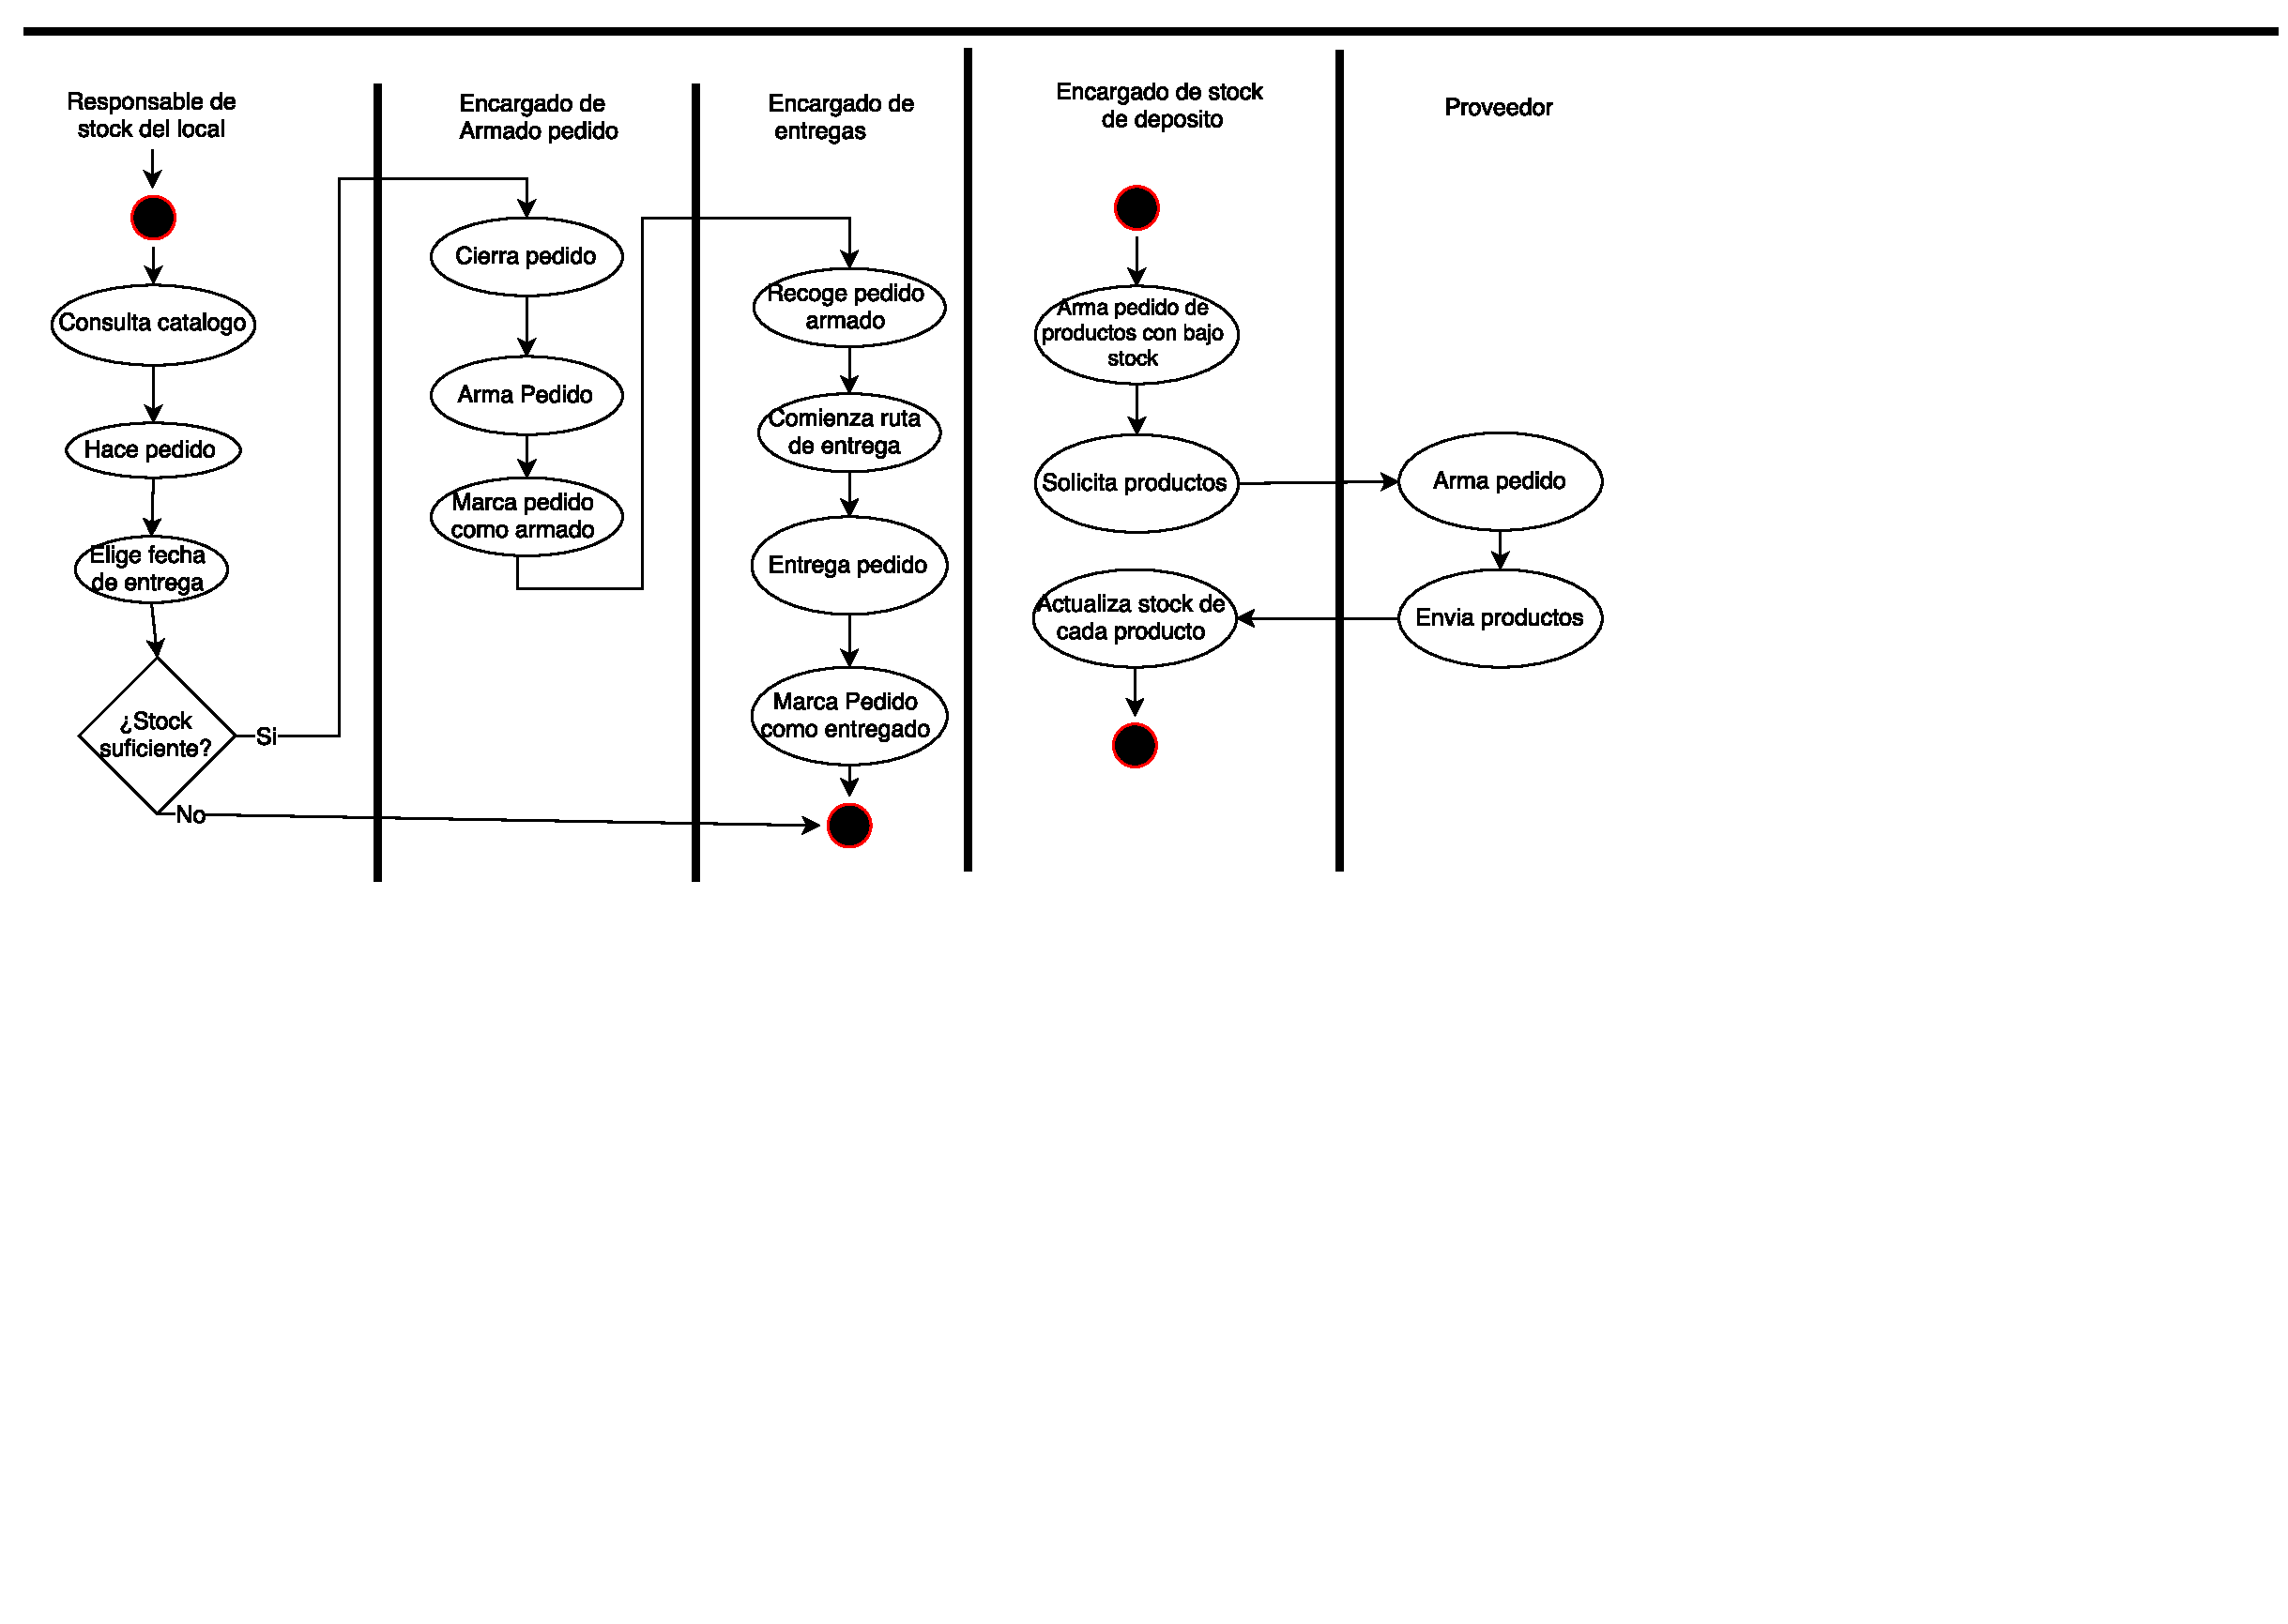
\includegraphics[scale=0.5, angle=90]{secciones/diagramaActividad2}

\newpage

\subsubsection{Trazabilidad}
A continuación listamos los requerimientos que se modelan con este diagrama.

\begin{itemize}
\item \textbf{Los usuarios se pueden autentificar:} Actividad loguearse
\item \textbf{Cerrar un pedido desde la pagina web:} Actividad Cierra pedido
\item \textbf{Tomar productos del pedido => Notificar pedido armado:} Actividad Marca pedido como armado
\item \textbf{Coordinar fecha de entrega:} Actividad Elije fecha
\item \textbf{Los locales pueden y ver y seleccionar los productos que desea recibir:} Actividad Consultar Catalogo
\item \textbf{Un cliente pueda seleccionar la fecha de entrega:} Actividad Elije fecha  de entrega
\item \textbf{Entregar pedidos al local:} Flujo de un pedido de un local
\item \textbf{Seleccionar pedido entregado:} Actividad Marca pedido como entregado
\item \textbf{El cliente pago en contra-entrega => se notifica pago a contra-entrega:} Actividad Paga pedido al contado
\item \textbf{El cliente pago desde la pagina => se notifica el pago online:} Actividad Loguearse en PayPal e Ingresando datos tarjeta
\item \textbf{Coordinar fecha de entrega con proveedor:} Actividad Solicita productos
\item \textbf{Ofrecer pago con PayPal:} Actividad Logueandose en PayPal
\item \textbf{Ofrecer pago con crédito:} Actividad Ingresando datos tarjeta
\item \textbf{Ofrecer pago con débito:} Actividad  Ingresando datos tarjeta
\item \textbf{Ofrecer pago con efectivo:} Actividad Paga pedido al contado

\end{itemize}

\newpage